\subsection*{---Functional Specifications}
At the beginning of the design phase, we set target functional specifications. We tried to make ambitious but attainable goals. Using the targets we were able to size the motor and amplifier we would need.In selecting a motor, a reference had to be used to run simulations, so a motor with torque constant of .11 N/m was used in tandem with an amplifier with a gain of .79 A/V. Using these sample motor and amplifier constants in the model, we ran simulations through Simulink to verify that such a motor amplifier combination would suffice by checking the maximum current, voltage, torque and rpm required against what the motor and amp could supply. Cases with low mass and damping proved to have the highest torque and current requirements because the velocity profile of such a system would involve very high accelerations. From the results we decided that damping must always be included in the reference system to limit the necessary torque.

After the design was finalized we developed a functional specification mapping to guide the user's inputs. The motivation for this was observing that the low mass, low damping case performed reasonably well as long as the force input was small. In addition, a greater force could be applied if either the damping or mass was increased. This led to the conclusion that the limitations on the reference system parameters were actually coupled. Considering the restrictions that either increasing the mass or the damping would put on the acceleration of the reference system for a given force input, this conclusion seemed logical. To create the mapping, we calculated the transfer function relating the force input to the required motor current.\begin{equation}
I = \frac{[K_{P}s+K_{I}][(\epsilon-M)s^{2}-Bs-K]}{[\frac{\epsilon}{K_{A}}s^{2}+\frac{K_{P}K_{M}}{r}s+\frac{K_{I}K_{M}N}{r}][Ms^{2}+Bs+K]}F
\end{equation}
Where 
\begin{equation}
\epsilon = M+\frac{JN^{2}}{r^{2}}
\end{equation}

\begin{figure*}[t]
	\centering
	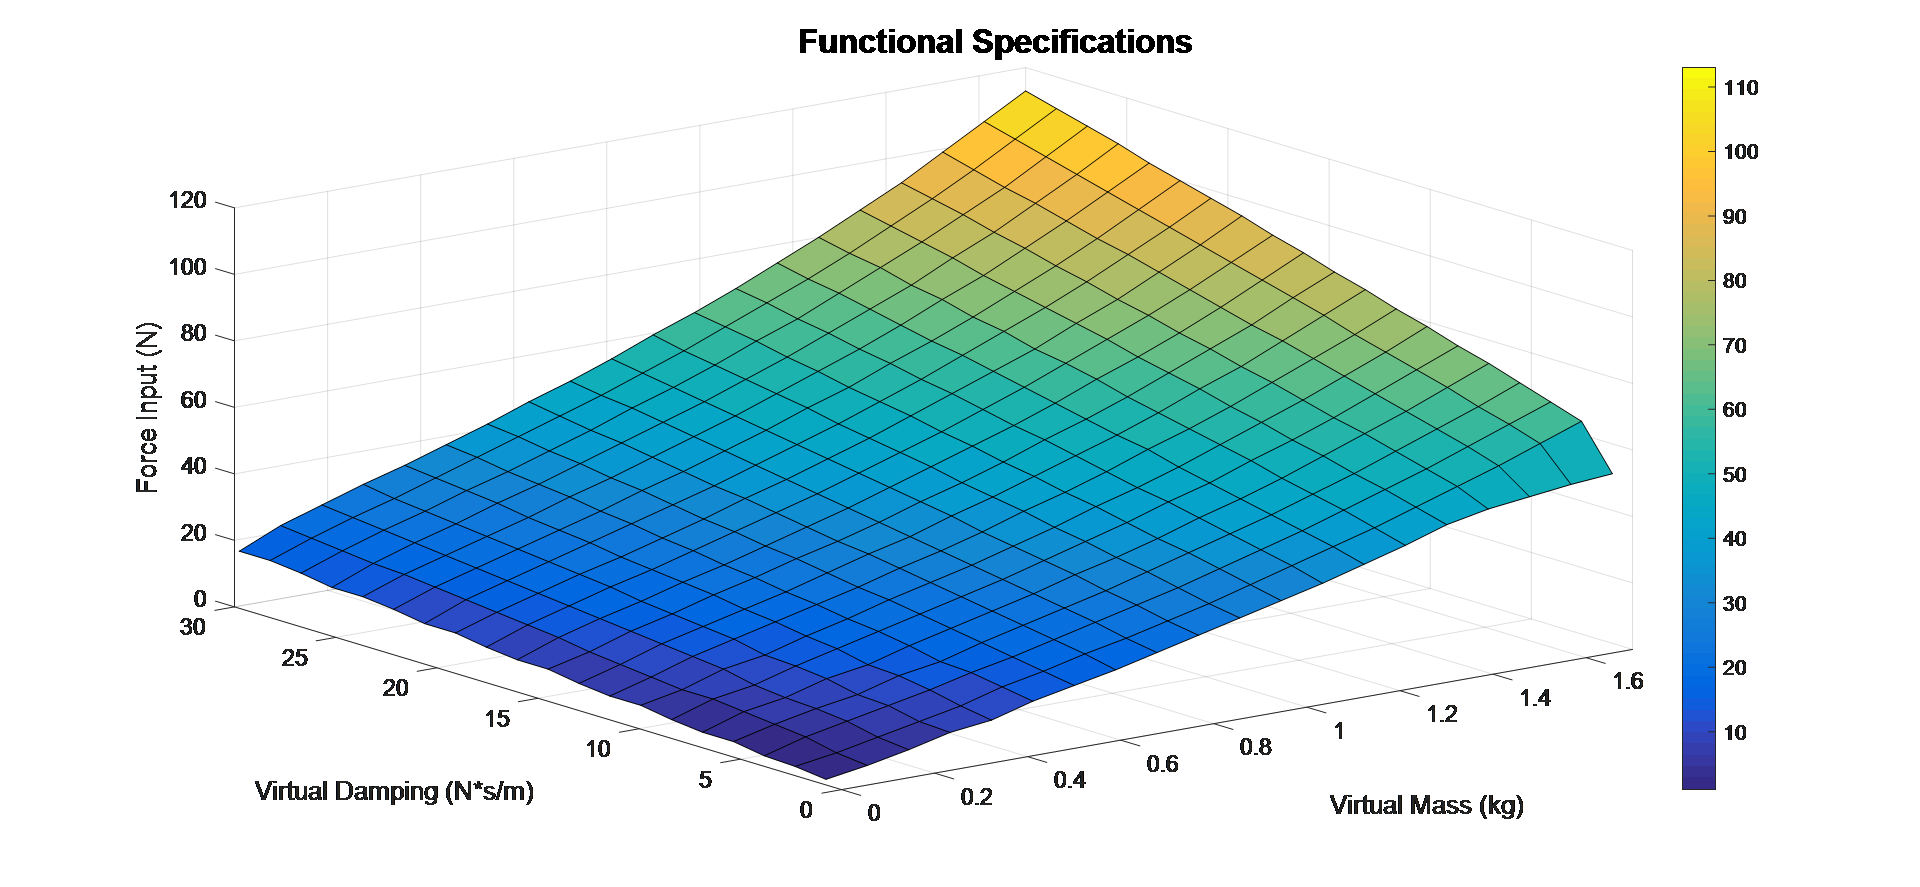
\includegraphics[width=1\linewidth]{../Functional_Specifications_Mapping}
	\caption{}
	\label{fig:Functional_Specifications_Mapping}
\end{figure*}
The transfer function depends on the parameters of both the reference and actual systems, as predicted, but not in any clearly identifiable way. The mapping was generated numerically using successive approximation to determine what applied force would result in the current requirement exceeding the limitations of the amplifier, about 4.8 A. The parameters varied were the mass and damping, as the relationship between the spring and acceleration was less complex and more intuitive and the input force was a critical component of any mapping.
The mapping shown is just a small portion of the effective range. We selected this portion because it demonstrates the very small force that can be applied when the reference system has very low mass and damping while showing the relationships between damping, mass and force. The maximum value of force shown is near 111 N which is approximately the limit of the load cell range. Theoretically, the force possible to apply would continue to increase beyond this point but the load cell would not read it as a greater force, so our system cannot handle greater forces regardless. If the load cell range was not the limiting factor, it is presumed that the force would increase with the damping and mass until the torque required to prevent the acceleration of the real system going beyond the reference system's response for the input force. In this way, the lower range of the the functional specification mapping can be seen as dependent on the ability of the motor to increase the acceleration of the real system and the higher range of the functional specification mapping can be seen as dependent on the ability of the motor to decrease the acceleration of the real system.